% !TeX root = ../manual.tex

\section{Tableaux de variation}

    Voir \href{https://zestedesavoir.com/tutoriels/439/des-tableaux-de-variations-et-de-signes-avec-latex/}{ce tutoriel}.

    \begin{latexcode}
        \begin{tikzpicture}
            \tkzTabInit[color]{$x$ / 1 , $f'(x)$ / 1, $f$ / 2} % Lignes (nom / taille)
            {$0$, $2$, $5$, $+\infty$}
            \tkzTabLine{z, -, d, h, d, +, }
            \tkzTabVar{+ / $13$, -DH / $4$,  D- / $\frac{\pi}{12}$, + / 15 }
            \tkzTabVal{3}{4}{0.5}{$\frac{\sqrt{333}}{2}$}{$7$}
        \end{tikzpicture}
    \end{latexcode}